\section{基于全局地图的高层导航方法}
\subsection{引言}
上述章节是在没有全局先验地图情况下对目标点进行追踪,并且在追踪过程中进行避障
等操作。当移动机器人具备了局部情况下的追踪与避障功能之后,这种基于局部点云的
算法只适合在小范围内进行导航,例如在学校的宿舍区或者食堂区域内局部活动。当给
定的目标点距离过远,超过局部点云的承载极限时(规划的目标点在点云之外),又或
者给定的目标点与移动智能机器人之间存在不可越过的障碍物时,例如园区内河、湖泊和
小山等,移动机器人无法得到障碍物后面的情况,只依赖当前局部规划算法的逻辑,根据
给定目标点的朝向和当前移动机器人的角度来单纯地局部规划,那么移动机器人便会陷入
局部最优之后——以局部算法的最优解去不停地尝试解决问题。这边会导致移动机器人始终
无法到达目标点。导航任务因此搁浅。

所以一旦涉及到园区的全局场景,上述底层导航功能便不再适用,当然一个可行的方法是在人为
事先采集好路点的情况下进行发布,并且由底层导航接收而后完成任务。那么为了弥补
这一导航系统的缺陷,势必需要对全局园区环境进行了解,并且在具有全局先验信息的
情况下,直接进行地图层级的规划,并且将规划得到的路径点逐一发布给底层导航,由
此完成整个导航任务。完成地图层级地规划需要几个先决条件,一是构建的全局地图,
用来存储全局的路径信息以及障地貌信息等;二是基于地图的路径规划算法,在地图上
规划处位于两个点之间的可行使路径,而后将规划得到的路径点发布出去。

\subsection{基于RTK的多层地图构建}
目前的建图算法十分多见,有基于SLAM系统的实时定位建图算法,可以在算法运行的同
时,实时地将地图建立起来,效率相比其他算法较高;也有基于全球定位系统、卫星定位
的离线建图方法。两种方法是目前比较主流的建图算法,且两者相比具有不同的优缺点。
前者效率较高,无需额外的定位设备,只需要激光雷达或者摄像头,比较典型的是LeGO\_LOAM
和ORB-SLAM为代表的SLAM算法。同时SLAM方法无需后期的人工拼接,但是在建图的精度上
不如后者;而基于卫星定位建图算法主要依赖是外部的定位设备,需要额外的成本,同时
必须进行人工后期拼接才能使用;但是它的优点也是极其明显的:可以人工拼接并做后期的
地图处理,同时具有较高的定位精度,也允许在一定程度上对地图进行编辑并在特定的算法
需求上提供不同的处理方案。在本实验是移动智能机器人的构建过程中,采购了中海达的高
精度车载组合定位模块,并且由于园区场景下,本着一次建图、永久使用的原则,无需重复
多次建图,因此综合建图精度、成本控制以及使用需求等多方面因素,最终决定使用基于高
精度车载组合定位系统(以下简称RTK)的方案进行园区场景的地图构建。

\subsubsection{点云地图}
为了建立多层次的全局地图,首先需要建立的是园区下的全局点云地图。点云的构建过程是
对采集到的点云按照位姿进行拼接以及对拼接后的地图进行后期处理的过程。为了在校园场景
下构建一幅适合移动智能机器人的导航系统,针对各个可供移动智能机器人通过的路径以及走
廊等位置进行数据采集,主要的采集平台是煜禾森公司的FR-07智能机器人底盘与装配的Velodyne
公司的VLP-16型激光雷达。关于此平台的参数将会在具体的硬件章节做更加深入的介绍。

在使用设备采集相应的点云信息之前,需要对车身以及设备之间的坐标系进行标定。标定后
的设备共有三大主要坐标系,分别是移动智能机器人底盘后轮中心的base\_link坐标系、
VLP-16激光雷达坐标系以及RTK坐标系。各个坐标系之间的相对位置关系如下图所示:
\begin{figure}[ht]
    \centering
    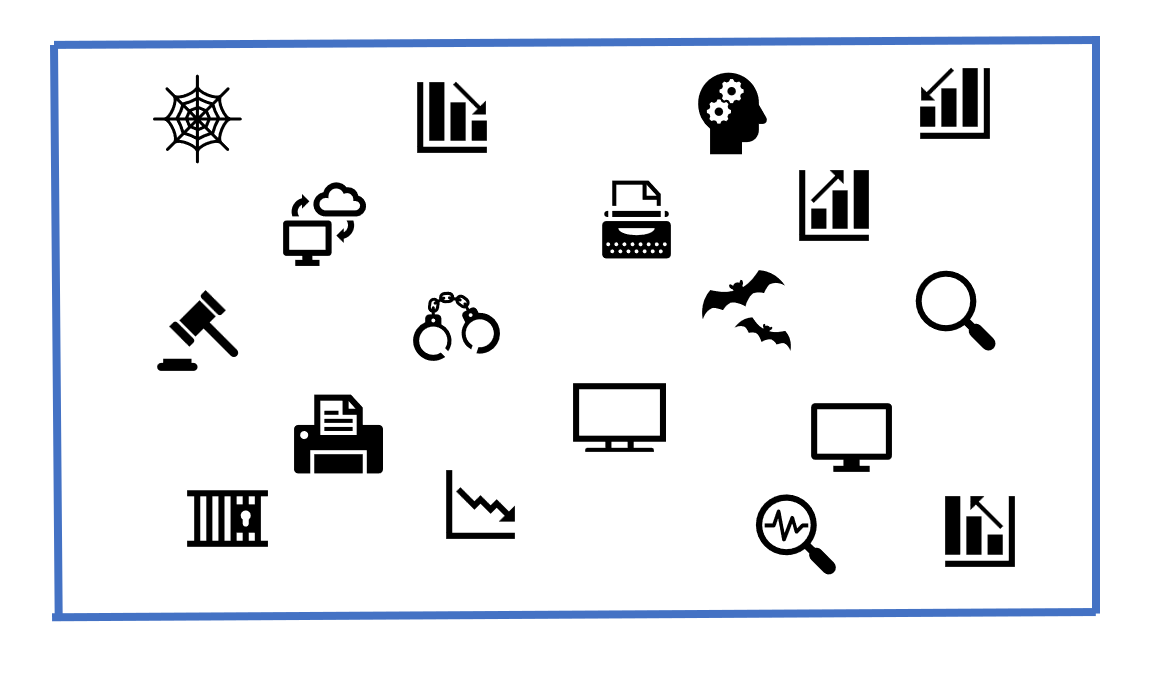
\includegraphics[scale=0.5]{template.jpg}
    \caption{模板图片}
\end{figure}

首先在园区全局内选定一处作为园区地图内的世界坐标系原点,考虑到整个地图的合理性,
选定的坐标系原点为校园中心位置。此处参考的地心坐标系统是WGS 84世界大地坐标系。
后续采集的点云数据均据此作为坐标系原点与位姿基准展开数据处理。

整个构建点云地图的流程框图如下所示:
\begin{figure}[ht]
    \centering
    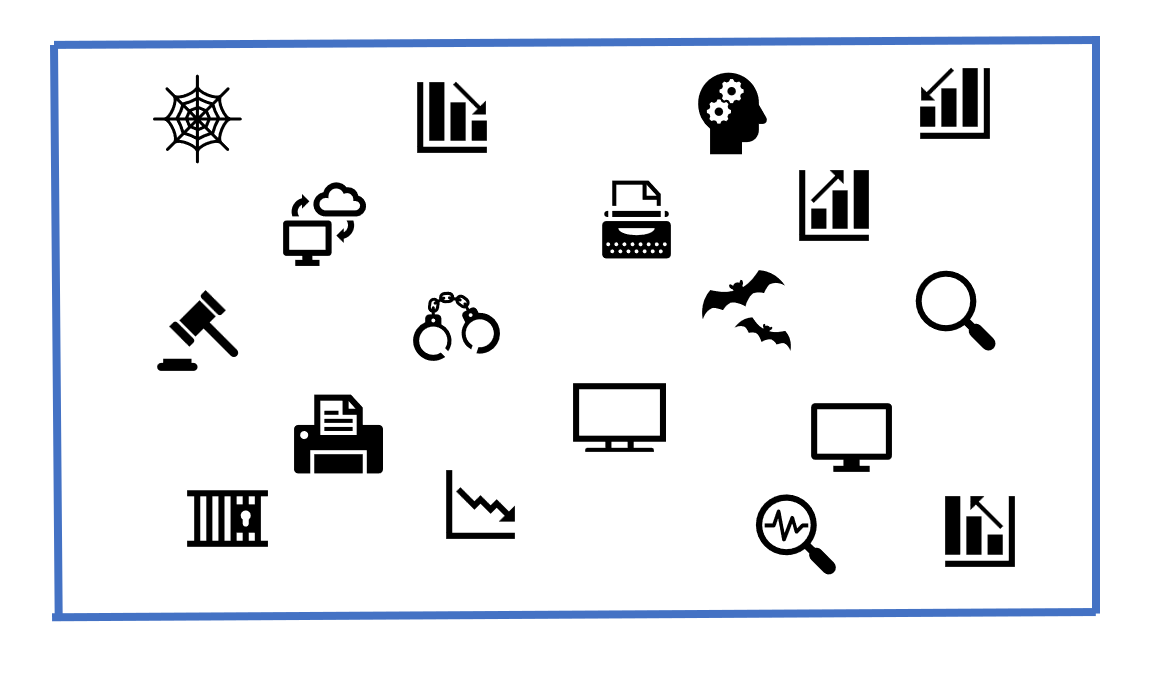
\includegraphics[scale=0.5]{template.jpg}
    \caption{模板图片}
\end{figure}

采集的软件系统为Robot Operating System(简称ROS系统)。采集地图的命令为:
sudo record -a;

\paragraph{地面提取}
地面提取的方式有多种,目前主流应用的是直接计算法、平面拟合法以及滤除法。其中直
接计算法是直接计算相邻两条激光线的俯仰角,俯仰角变化在一定范围内的可以被认为是
地面点;平面拟合法在底层导航一章中已经有叙述,主要是通过选取种子点拟合出相应平
面,并且通过迭代方法使得地面选取更加精准。再全局地图的构建过程中,由于不再是之
前简单将地面点去除,只需要迭代出地面后去除即可,关注点在于非地面点。此时我们对
于点云中地面点的质量有了更高的要求,是“宁缺毋滥”地筛选符合要求地地面点,人为增
加了点的筛选门槛。下面给出具体方法。
对采集得到的点云包进行分析,找到其中的velodyne\_points话题,对于包中所含有的
任意一帧点云进行分析,提取其中的非地面点部分与地面部分。提取地面部分点云的方法
如下所示:
对于激光雷达采到的任意一点,此点与激光雷达的位置关如下图所示:
\begin{figure}[ht]
    \centering
    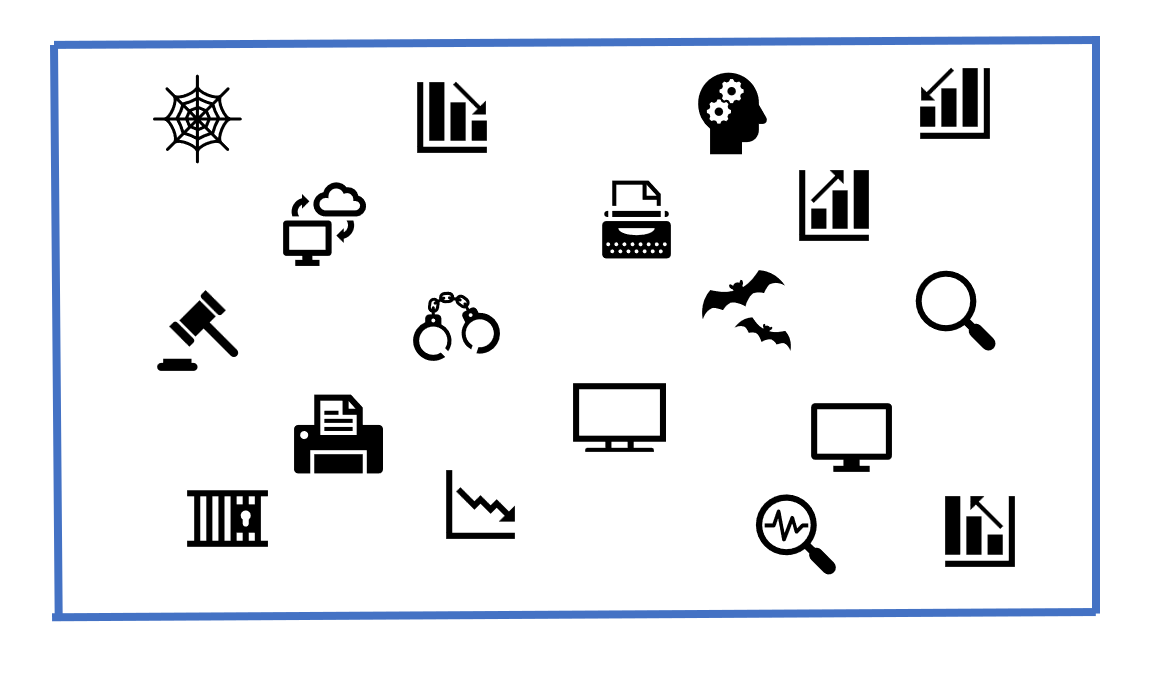
\includegraphics[scale=0.5]{template.jpg}
    \caption{模板图片}
\end{figure}

在激光雷达坐标系中,$\theta$ 表示点与水平xoy平面的夹角,x、y、z分别表示到坐标轴的距离
首先根据公式
\begin{equation}
    radius = \sqrt{x^2 + y^2}
\end{equation}
计算点的采集半径radius,再根据
\begin{equation}
    \theta = atan2(z ,radius) * 180 / \pi 
\end{equation}
计算得到点与水平面的夹角,atan2函数的象限划分与对应角度不同于atan函数,其原理为
\begin{equation}
\operatorname{atan} 2(y, x)=\left\{\begin{array}{ll}
    \arctan \left(\frac{y}{x}\right) & x>0 \\
    \arctan \left(\frac{y}{x}\right)+\pi & y \geq 0, x<0 \\
    \arctan \left(\frac{y}{x}\right)-\pi & y<0, x<0 \\
    +\frac{\pi}{2} & y>0, x=0 \\
    -\frac{\pi}{2} & y<0, x=0 \\
    \text { undefined } & y=0, x=0
    \end{array}\right.
\end{equation}

低于激光雷达坐标系xoy平面的点角度判定为-,而高于此平面的点角度判定则为+。
得到了某点的角度$\theta$,根据VLP-16激光雷达的角度分布,便可以得到某点所属于的
扫描线序号scanID,根据地面扫描点主要集中于最下面的三条扫描线的特点,只取角度为
-15°、-13°、-11°的三条扫描线上的点进行分析。
根据scanID将属于某条扫描线的点集合起来,检测点的粗糙值,粗糙值的计算公式为
\begin{equation}
    c_i=\frac{1}{|P|}\sum_{j\in P, j \ne i }||p_i-p_j|| 
\end{equation}
表达式的意思是首先取当前点同scanID的前后各十个点,$c_i$表示当前点的平滑度,P表示
当前点与其前后十点的集合,|P|值为邻点的数量,$p_i$、$p_j$分别表示当前点的向量与
其邻点的向量,对向量取2-范数。最终的平滑度表示为当前点与其周围——同一扫描线前后各10
点之间的距离均值。
并且在最后对下三线上的点完成分析之后,设置相应阈值,使得地面点合格率约为1/3左右。
最终,通过此方法取得的地面点在保证了点密度的情况下最大限度保证了地面点的质量。

\paragraph{基于RTK的地图合成}
每一帧地面点云地数据拿到之后,需要对地面点云根据位姿进行拼接,拼接点云地位姿来源于
数据采集过程中同时间戳录制的RTK位姿数据。
在前面fast\_gicp的叙述中也有提到两帧不同位姿的数据如何进行拼接,其实就是统一坐标系的
过程。与之前不同的是,之前的拼接没有一个全局的参考坐标系,是对车身位置实时位姿变换。
当在园区场景内选定了全局坐标系之后,若某一帧点云的位姿相对于全局位姿的变换为R、t,分
别表示点云帧相对于全局位姿所作的旋转与平移。
任意时刻,某点与当前坐标系的位置示意图如下所示。
\begin{figure}[ht]
    \centering
    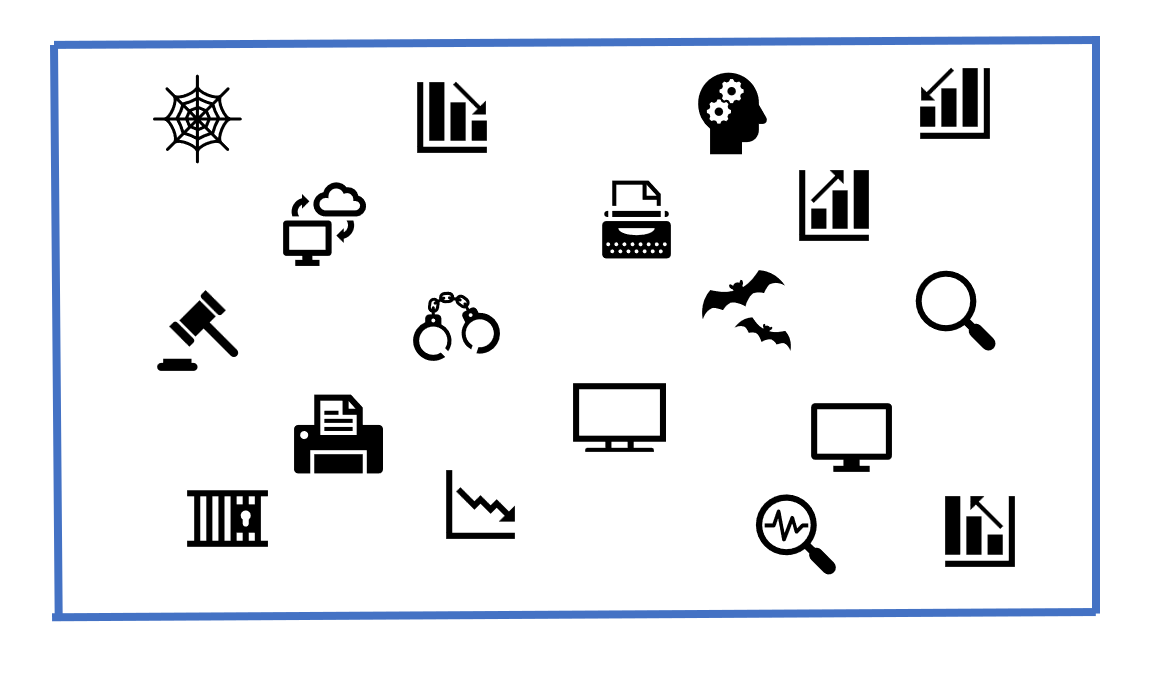
\includegraphics[scale=0.5]{template.jpg}
    \caption{模板图片}
\end{figure}
将当前点云中某点变换到全局坐标系下的变换为
\begin{equation}
    P'_1 = \symbf{R} * P_1 + \symbf{t}
\end{equation}


$P_1$表示点云的中某点的向量$[x,y,z]^T$,当前位姿,$P'_1$表示变换到全局坐标系下的位姿$[x',y',z']^T$。
该式还可以通过齐次坐标和变换矩阵的形式表现
\begin{equation}
    \begin{aligned}
    P'_2 = \symbf{T} * P_2 \\
    T=\begin{bmatrix}
        R& t\\
        0^T&1
      \end{bmatrix}
    \end{aligned}
\end{equation}
$P_2$表示点云的中某点的向量$[x,y,z,1]^T$,当前位姿,$P'_2$表示变换到全局坐标系下的位姿$[x',y',z',1]^T$。

此处可以直接调用pcl::transformPointCloud将一帧地面点云位姿变换到全局坐标系下,此过程仍然需要在一定帧数
拼接完成后进行降采样操作。操作原理与上一章类似。至此,地面点云的点云地图拼接完成,效果如下所示。
\begin{figure}[ht]
    \centering
    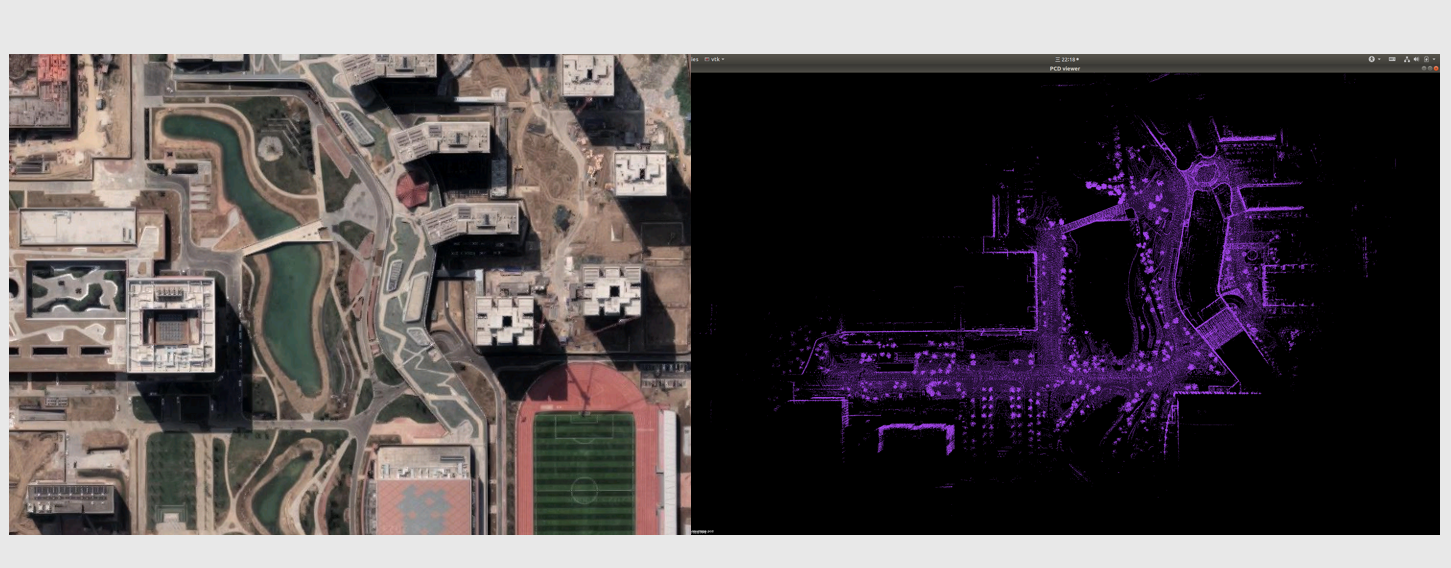
\includegraphics[scale=0.45]{globalPointsMap1.png}
    \caption{全局点云地图与原图片对比}
\end{figure}

\textcolor{red}{\underline{可以添加一部分用来讨论WSG84到RTK站心坐标系的转换}}

\subsubsection{栅格地图}
在得到了上述的地面点云地图roadMapAll之后,开始需要对这些可行使区域进行栅格化。在实际使用过程中,栅格化不必要对整个点云
地图进行,只需要对需要的可行驶区域部分,也就是上述得到的地面点云地图进行栅格化操作。
第一步获得此roadMapAll中点的极限值——所有点中最小的x值,y值,z值以及最大的x值,y值,z值。
依据此值对整个roadMapAll区域进行划分,按照0.5*0.5m的分辨率得到相应的栅格地图,每一个方格内所有点的平均高度为gridAverageHeight;


\paragraph{泛洪算法}
接下来使用著名的泛洪算法中的四邻域泛洪法,

\paragraph{腐蚀算法}
腐蚀算法主要目的是刻蚀掉孤悬于主区域之外的零星可行驶区域,此区域与其他可行驶区域的连接性不强,我们是不希望它作为后续路径规划的
节点网格的。





\subsection{基于距离地图的全局路径规划算法}
在选定的栅格地图基础上,进行全局的路径规划,规划时不考虑全局地图上的动态性,默认全局地
图上的可行驶区域在规划时刻均为静态可通行。一般来说,全局规划的算法有很多种,例如RRT、
RRT*、A*、Hybird A*、D*、Dijkstra等等。其中RRT簇适用于随机规划路径,但规划出的路径
不是最优的;A*簇算法适用于具备全局地图情况下的规划,并且规划出的路径是最优路径,其衍生
算法D*可以在地图有改变的情况下进行局部重规划;Dijkstra算法是一种BFS式的搜索算法,与A*类
算法相比,具有较高的搜索代价。由于我们提前说明不考虑全局地图上的动态性,故在全局搜索中
使用的是A*规划算法。

\subsubsection{A*算法}
原理简述:A星算法是一种常用于寻路问题的算法,可以在图形图像中找到从一个起点到一个目标点
的最短路径。一共如下3大步骤:
初始化起点和终点:首先将起点加入open列表,open列表存放所有待考虑的节点。同时初始化g值
和h值,其中g值是起点到当前节点的距离,h值是当前节点到终点的估计距离(如欧几里得距离)。

循环直到找到终点:在每次循环中,从open列表中选取f值最小的节点作为当前节点,并将其移入
closed列表中。如果当前节点为终点,则搜索完成。否则,将当前节点的邻居节点(即可以直接到
达的节点)加入open列表中,计算它们的g和h值。如果邻居节点已经在closed列表中,或者g值更
大,则不做处理。否则,更新g值,重新计算f值。

最终路径的生成:当终点被找到时,从终点开始按照每个节点的父节点反向寻找路径,直到回到起
点为止。这就是从起点到终点的最短路径。
A星算法的优点在于可以通过启发式函数对估计的距离进行优化,使得算法能够快速找到最短路径。同时,算法能够在不考虑地形的情况下进行路径规划,这使得它在游戏设计、机器人路径规划等领域得到了广泛应用。

A*算法的问题可以描述为
\begin{figure}[ht]
    \centering
    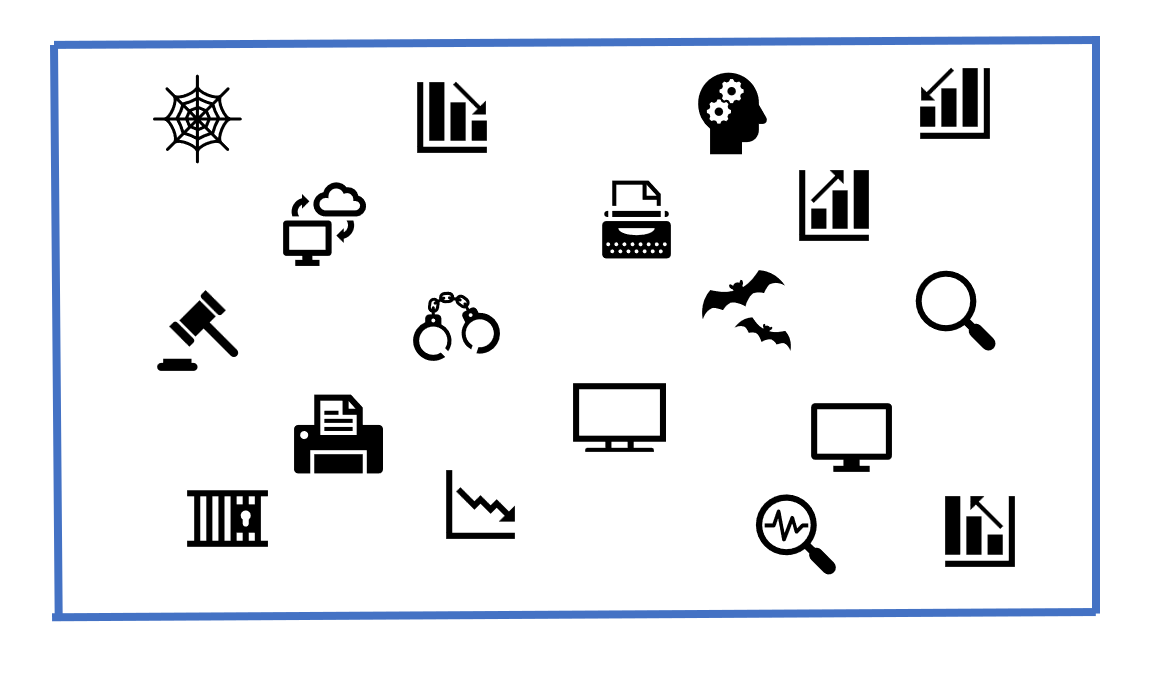
\includegraphics[scale=0.5]{template.jpg}
    \caption{模板图片}
\end{figure}

如何穿过避开障碍物并且在最小消耗的情况下到达终点位置。

在A*算法中最重要的是启发函数的设置,通常规律下,A*算法的启发函数可以描述为
\begin{equation}
    F = \alpha G +\beta  H
\end{equation}
其中,F表示总代价

G = 从起点 A 移动到指定方格的移动代价,沿着到达该方格而生成的路径。
H = 从指定的方格移动到终点 B 的估算成本。这个通常被称为试探法,因为
这是个猜测。直到我们找到了路径我们才会知道真正的距离,因为途中有障碍物
阻挡于当前网格节点与终点之间。
通过调节G与H的系数$\alpha$、 $\beta$ 可以对搜索的方式进行调整。例如当在距离地图中希望规划出的路径远离地图场景中
本就存在的障碍物时,便可以将H调整为到终点的估算成本与周围障碍物距离的加权和。

